\documentclass[12pt]{article}

\usepackage[utf8]{inputenc}
\usepackage[T1]{fontenc}
\usepackage{lmodern}
\usepackage{amsmath, amssymb}
\usepackage{graphicx}
\usepackage{hyperref}
\usepackage{geometry}
\usepackage{fancyhdr}
\usepackage{enumitem}
\usepackage{listings}
\usepackage{xcolor}
\usepackage{algorithm2e}
\usepackage{algorithmicx}
\usepackage{tcolorbox}
\usepackage{amsmath}
\usepackage{amsthm}
\usepackage{amsfonts}
\usepackage{amssymb}
\usepackage{setspace}

\lstset{
  language=C++,
  basicstyle=\ttfamily\small,
  keywordstyle=\color{blue}\bfseries,
  stringstyle=\color{red},
  commentstyle=\color{gray},
  morecomment=[l][\color{magenta}]{\#},
  numbers=left,
  numberstyle=\tiny\color{gray},
  stepnumber=1,
  numbersep=10pt,
  backgroundcolor=\color{white},
  showspaces=false,
  showstringspaces=false,
  emph={int,float, double},
  frame=single,
  tabsize=4,
  breaklines=true,
  emphstyle=\color{purple},
  escapeinside={*@}{@*}
  }
% escapechar=|,


\tcbuselibrary{theorems, skins, breakable}

\newtcbtheorem[auto counter, number within=section]{TheoremColor}{Theorem}%
{colback=red!10!white,colframe=red!100!black,fonttitle=\bfseries, separator sign none,
left=2pt,right=2pt,top=2pt,bottom=2pt,
width=1.02\linewidth,
theorem style=plain,
code={\onehalfspacing},
%separator sign={\ $\blacktriangleright$},
description delimiters parenthesis, description color=red!25!purple,
coltitle=blue!75!black}{th}

\newtcbtheorem[use counter from=TheoremColor]{TheoremColorTitle}{Theorem}%
{colback=red!10!white,colframe=red!100!black,fonttitle=\bfseries, separator sign none,
left=2pt,right=2pt,top=2pt,bottom=2pt,
width=1.02\linewidth,
code={\onehalfspacing},
description delimiters parenthesis, description color=black!100!white,
coltitle=blue!75!black}{th}


\newtcbtheorem[use counter from=TheoremColor]{LemmaColor}{Lemma}%
{colback=green!10!white,colframe=green!100!black,fonttitle=\bfseries, separator sign none,
left=2pt,right=2pt,top=2pt,bottom=2pt,
theorem style=plain,
width=1.02\linewidth,
code={\onehalfspacing},
description delimiters parenthesis, description color=red!25!purple,
coltitle=blue!75!black}{le}

\newtcbtheorem[use counter from=TheoremColor]{CorollaryColor}{Corollary}%
{colback=orange!10!white,colframe=orange!50!black,fonttitle=\bfseries, separator sign none,
left=2pt,right=2pt,top=2pt,bottom=2pt,
theorem style=plain,
width=1.02\linewidth,
code={\onehalfspacing},
description delimiters parenthesis, description color=red!25!purple,
coltitle=blue!75!black}{cor}


\newtcbtheorem[use counter from=TheoremColor]{DefinitionColor}{Definition}%
{colback=yellow!10!white,colframe=yellow!75!black,fonttitle=\bfseries,
left=2pt,right=2pt,top=2pt,bottom=2pt,
width=1.02\linewidth,
theorem style=plain,
code={\onehalfspacing},
description delimiters parenthesis, description color=red!25!purple,coltitle=blue!75!black}{def}

\newtcbtheorem[use counter from=TheoremColor]{DefinitionColorBreak}{Definition}%
{colback=yellow!10!white,colframe=yellow!75!black,fonttitle=\bfseries,
left=2pt,right=2pt,top=2pt,bottom=2pt,
width=1.02\linewidth,
theorem style=plain,
breakable,
code={\onehalfspacing},
description delimiters parenthesis, description color=red!25!purple,coltitle=blue!75!black}{def}

\tcolorboxenvironment{proof}{% `proof' from `amsthm'
blanker, breakable, left=3mm,
width=1.02\linewidth,
code={\onehalfspacing},
before skip=10pt, after skip=10pt,
before upper={\parindent15pt\noindent},
borderline west={1mm}{0pt}{blue}}



\BeforeBeginEnvironment{DefinitionColor}{\savenotes}
\AfterEndEnvironment{DefinitionColor}{\spewnotes}

\BeforeBeginEnvironment{DefinitionColorBreak}{\savenotes}
\AfterEndEnvironment{DefinitionColorBreak}{\spewnotes}


\geometry{a4paper, margin=1in}
\pagestyle{fancy}
\fancyhf{}
\rhead{\thepage}
\lhead{Djordje Zivanovic}

\title{Next Silicon: CM Home Assignment}
\author{Djordje Zivanovic \\ \small{LinScale}}
\date{\today}

\begin{document}

\maketitle
\tableofcontents
\newpage

\section{Introduction}
This report \footnote{\href{https://github.com/popina1994/Next-Silicon-Report}{report}} contains the responses to the tasks stated in the home project pdf.
It is accompanied with the repository \footnote{\href{https://github.com/popina1994/next-silicon-maths}{next-silicon-maths}} that contains reproducible solutions with the installation instructions alongside: experiments and tests according to the task requirements.
\section{The Existing Implementation: Code Analysis and Documentation}
In this section we analyze the existing code shown in Algorithm \ref{alg:sine_existing}.

\subsection{Code Drawbacks}
The code is written for C and follows the following bad practices and readability improvements:
\begin{enumerate}
    \item Reusing the variable multiple times,  \texttt{(float)M\_PI} and \texttt{2.0f * (float)M\_PI}, (lines \ref{alg:sine_ex:ln:fmodf}, \ref{alg:sine_ex:ln:xGreater}, \ref{alg:sine_ex:ln:xLess}, \ref{alg:sine_ex:ln:xLess}, \ref{alg:sine_ex:ln:xMinus}, \ref{alg:sine_ex:ln:xPi} of Algorithm \ref{alg:sine_existing});
    \item Not using auto in order to automatically deduce types since the results of all the statements are known;
    \item Cleaning if loop to be more understandable: \texttt{fmodf} returns the result in the range $(-2 \pi, 2 \pi)$. Then, now it is obvious that one checks whether the number is outside of the range $[-\pi, \pi]$, and then updates \textbf{x} for $2 \pi$ period, so the further code operates with the number in the range $[-\pi, \pi]$;
    \item Adding more verbosity with names and code structure;
    \item Reusing variable names -> more verbose names should be used in order to improve readability of the code. The c ompiler will optimize for the least number of variables/registers to be used;
    \item Renaming function names and migrating these functions to the corresponding headers and sources that would contain the custom maths functions.
\end{enumerate}


\begin{algorithm}
    \caption{Algorithm with Code Listing}
    \begin{algorithmic}[1]
    \State \textbf{Input:} A float (IEEE-754) number
    \State \textbf{Output:} A float (IEEE-754) sine value of this number computed using Taylor Series.
    \State \textbf{Steps:}
\begin{lstlisting}[numbers=left]
float fp32_custom_sine(float x)
{
    x = fmodf(x, 2.0f * (float)M_PI);  *@\label{alg:sine_ex:ln:fmodf}@*
    if (x > (float)M_PI) *@\label{alg:sine_ex:ln:xGreater}@*
        x -= 2.0f * (float)M_PI; *@\label{alg:sine_ex:ln:xMinus}@*
    else if (x < -(float)M_PI) *@\label{alg:sine_ex:ln:xLess}@*
        x += 2.0f * (float)M_PI; *@\label{alg:sine_ex:ln:xPi}@*
    float result = 0.0f;
    float term = x;
    float x_squared = x * x;
    int sign = 1;
    for (int n = 1; n <= 7; n += 2)
    {
        result += sign * term;
        sign = -sign;
        term = term * x_squared;
        term = term / (float)(n + 1);
        term = term / (float)(n + 2);
    }
    return result;
}

\end{lstlisting}
\end{algorithmic}
 \label{alg:sine_existing}
\end{algorithm}

\subsection{Numerical and Implementation Drawbacks}
Here, I will give state several main drawbacks in terms of the implementation and numerical accuracy.
\begin{enumerate}
    \item Reducing number of \texttt{2.0f * M\_PI} computations;
    \item Expressing \texttt{2.0f * M\_PI as 2 * M\_PI} -> this should be expressed as a sum of two \texttt{M\_PIs}
    \item Transforming \texttt{term = term / (n + 1)} and then \texttt{term = term / (n+2)} to \texttt{term= term / ( (n+1) *(n+2))}. Instead of two float divisions and two stores, these are two integer additions (tend to be faster) and only one float division and one store.
    \item Unrolling the loop by starting from \texttt{n = 3}, we know the first element will always be \texttt{x}. We can thus skip the computations in the loop for n =1. We also, do not need to compute the next term in advance, only for the current n. Thus we are saving the computations after result updated (sign change, and term updating).
    \item we also can accumulate the divisions by integers in a variable.
    \item  sign multiplication by the term, can be replaced by if else in order to avoid on FLOP for \texttt{sign * term}.
\end{enumerate}

In the next subsection, I will list the drawbacks related to the method itself.
\subsection{Mathematical Analysis}
Let us state the general Taylor series formula that is implemented in Algorithm \ref{alg:sine_existing}.
\begin{TheoremColor}{Theorem 5.19 from \protect{\cite[p.~113]{apostol1985mathematical}}}{taylor_formula}
    Let $f$ be a function having finite $n$-th derivative $f^{(n)}$
    everywhere in an open interval $(a, b)$ and assume that  $f^{(n-1)}$ is continuous on the closed interval $[a, b]$. Then, for every $x$ in $[a, b], x\neq c$, there exists a point $x_1$ interior to the interval joining $x$ and $c$ such that

    \begin{equation*}
        f(x) = f(c) + \sum_{k=1}^{n-1} \frac{f^{(k)}(c)(x-c)^{(k)}}{k!} + \frac{f^{(n)}(x_1)}{n!} (x - c)^n.
    \end{equation*}
\end{TheoremColor}
A corollary of Theorem \ref{th:taylor_formula} when we set $c = 0$ is a Maclaurin Series.
\begin{CorollaryColor}{Maclaurin Series}{Maclaurin}
    Let $f$ be a function having finite $n$-th derivative $f^{(n)}$
    everywhere in an open interval $(a, b)$ and assume that  $f^{(n-1)}$ is continuous on the closed interval $[a, b]$. Assume that $c \in [a, b]$. Then, for every $x$ in $[a, b], x\neq 0$, there exists a point $x_1$ interior to the interval joining $x$ and $0$ such that

    \begin{equation*}
        f(x) = f(0) + \sum_{k=1}^{n-1} \frac{f^{(k)}(0)(x)^{(k)}}{k!} + \frac{f^{(n)}(x_1)}{n!} x^n.
    \end{equation*}
\end{CorollaryColor}
Let us now set $a = -\pi, b= \pi$ and $f(x) = sin(x)$ .
The Maclaurin Series becomes for $\sin$ function:
\begin{CorollaryColor}{}{sine_mac}
    For $x \in \mathbb{R}, x\neq 0$ and $n \in \mathbb{N}$, and $0 < |x_1| < |x|$
    the approximation of a degree $n$ is
    \begin{equation*}
        sin(x) = \sum_{i=0}^{\lfloor\frac{n}{2}\rfloor}
        \left(-1\right)^{ i} \frac{x^{2i + 1}}{(2i+1)!}   +  L(x, n).
    \end{equation*}
    where
    \begin{equation*}
        L(x, n) = \begin{cases}
            \frac{f^{(n + 2)}x_1}{(n+2)!}x^{n+2}, & \text{if } n \bmod 2 = 0,  \\
            \frac{f^{(n + 1)}x_1}{(n+1)!}x^{n+1}, & \text{if } n \bmod 2 = 1.
          \end{cases}
    \end{equation*}
\end{CorollaryColor}
Thus, the method stated in Algorithm \ref{alg:sine_existing} has an algorithmic error $L(x, 7)$ which is smaller than $\frac{x^8}{8!}$. However, for large numbers this can be quite huge.

\subsection{Accuracy and Correctness Failures} \label{subsec:acc_and_corr}
Based on Corollary \ref{cor:sine_mac}, we can notice that Algorithm \ref{alg:sine_existing} is incorrect for $x = 0$.
Similar, the farther $x$ is from 0, the error is larger since $x^8$ grows exponentially.
There are several ways to solve these problems:

\subsection{Experiments}


The test plan will cover the following experiments:
\begin{enumerate}
    \item Different number distributions
    \begin{enumerate}
        \item Equally distanced numbers between certain multiplicands of $\frac{\pi}{2}$; We will vary the distance and provide statistical analysis with plots for each of such distance and multi`plicand.
        \item Normally distributed numbers around certain multiplicands of $\frac{\pi}{2}$; We will vary the variance and provide statistical analysis with plots for each of the multiplicands and variances.
    \end{enumerate}
    \item Edge cases
        \begin{enumerate}
            \item the multiplicands of $\frac{\pi}{2}$;
            \item large numbers (larger than ULP);
            \item normal distributions around the multiplicands of $\frac{\pi}{2}$;
            \item \texttt{nan}s.
        \end{enumerate}
\end{enumerate}
For each of these experiments we would compute the relative error in comparison to the value computed by the $\sin x$ provided in \texttt{cmath}.
\newpage
\section{Additional Algorithms}
Here we list the additional algorithms we have chosen.
\subsection{Preliminaries and Implementation}
For the problems stated in Subsection \ref{subsec:acc_and_corr} there are several ways to approach:
\begin{enumerate}
    \item Have another Taylor series expansion for numbers around $\pi$ and $-\pi$. In this case we would manually calculate the $\sin x$ for $\pi$ and $-\pi$.
    \item  Add more terms in Taylor series expansion. It is important to find the optimal degree for the balance of accuracy and performance.
    \item Implement one or more of the alternative methods: Minimax Polynomial Approximation, Chebyshev Polynomial Expansion \cite{press2007numerical}, Lookup Table with Linear Interpolation and Lookup Table with Spline or Cubic Interpolation.
\end{enumerate}
In Algorithm \ref{alg:tay_optimized}, all the downsides listed in the previous section with regards to the provided implementation have been fixed.
In particular, we added more terms and optimized the existing code.

\begin{algorithm}
    \caption{Sine using Taylor series: Optimized Method}
    \begin{algorithmic}[1]
    \State \textbf{Input:} A float (IEEE-754) number and the degree \texttt{degreeEnd} used in Taylor series.
    \State \textbf{Output:} A float (IEEE-754) sine value of this number computed using Taylor series.
\begin{lstlisting}[numbers=left]
    float nextSiliconSineFP32Taylor(float x, uint32_t degreeEnd)
    {
        static constexpr auto PI_F = pi_v<float>;
        static constexpr auto TWO_PI_F = 2 * PI_F;
        static constexpr auto TAYLOR_DEGREE_START = 3u;
        static constexpr auto TAYLOR_DEGREE_NEXT_INC = 2u;

        if (std::abs(x) == 0.f) { return 0; }

        auto xPiRange = fmodf(x, TWO_PI_F);
        if (std::abs(xPiRange) > PI_F)
        { xPiRange -=  boost::math::sign(xPiRange) * TWO_PI_F; }

        auto result = xPiRange;
        auto term = xPiRange;
        const auto xPiRangeSquared = xPiRange * xPiRange;
        auto sign = 1;
        std::vector<float> vFact(degreeEnd + 1, 0);
        vFact[1] = 1;

        for (auto taylorDegree = TAYLOR_DEGREE_START;
            taylorDegree <= degreeEnd;
            taylorDegree += TAYLOR_DEGREE_NEXT_INC)
        { vFact[taylorDegree] = vFact[taylorDegree - 2] * (taylorDegree - 1) * taylorDegree;}

        for (auto taylorDegree = TAYLOR_DEGREE_START;
            taylorDegree <= degreeEnd;
            taylorDegree += TAYLOR_DEGREE_NEXT_INC)
        {
            sign = -sign;
            term = term * xPiRangeSquared;
            auto termAdd = term / float(vFact[taylorDegree]);
            if (sign == 1)
            {
                result += termAdd;
            }
            else
            {
                result -= termAdd;
            }
        }

        return result;
    }

\end{lstlisting}
\end{algorithmic}
 \label{alg:tay_optimized}
\end{algorithm}.
Here we will focus on the implementation of the Chebyshev Polynomial Expansion.

\begin{DefinitionColor}{\cite[p~.233]{press2007numerical}}{cheb_poly}
    For a number $n\in \mathbb{N}$ and a real number $x$, the Chebyshev polynomial of degree $n$ is denoted $T_n(x)$ and defined as
    \begin{equation*}
        T_n(x) = \cos(n \arccos x).
    \end{equation*}
\end{DefinitionColor}

\begin{TheoremColor}{}{cheb_rec}
    For $n \in \mathbb{N}$,and $x \in \mathbb{R}$ the Chebyshev polynomial of degree $n$ satisfies the formula:
    \begin{equation*}
        T_n=2xT_n(x) - T_{n-1}(x),
    \end{equation*}
    where $T_0(x) =1$ and $T_1(x) = x$.
\end{TheoremColor}
Let us introduce definitions that would help with our computations.

\begin{DefinitionColor}{\cite[p~.234]{press2007numerical}}{cheb_coef}
    For a number $j, N\in \mathbb{N}$, the Chebyshev coefficient of degree $n$ is denoted $c_n(x)$ and defined as
    \begin{equation*}
        c_j(N) = \frac{2}{N} \sum_{k=0}^{N-1} f\left( \cos\left(  \frac{\pi(k+\frac{1}{2})}{N}\right)  \right) \cos \left(\frac{\pi j(k+\frac{1}{2})}{N}\right).
    \end{equation*}
\end{DefinitionColor}

Now the following formula holds:
\begin{TheoremColor}{}{cheb_approx}
    Let $N \in \mathbb{N}$, $x \in \mathbb{N}$, and a function $f : [-1, 1] \mapsto \mathbb{R}$.
    Let $f$ be a continuous and bounded function. Now, the follows holds:
    \begin{equation*}
        f(x) \approx \sum_{k=0}^{N-1} \left(c_k(N) \cdot T_k(x)\right) - \frac{1}{2} c_0(N).
    \end{equation*}
\end{TheoremColor}

We implement the approximation from Theorem \ref{th:cheb_approx} in Algorithm \ref{alg:sine_cheb_opt}.
Chebyshev coefficients are computed in Algorithm \ref{alg:cheb_coef}.
Since Chebyshev coefficients from Definition \ref{def:cheb_coef} are defined for the input $[-1, 1]$, but our input is in the range $[-\pi, \pi]$, we need to map the input to $[-1, 1]$ by uniformly scaling the input to this range (Algorithm \ref{alg:sine_cheb_opt} line \ref{alg:sine_cheb:ln:scaling}).
However, we have to scale back the input to $[-\pi, \pi]$ for the function $\texttt{f}$ in Algorithm \ref{alg:cheb_coef} (lines \ref{alg:sine_cheb:ln:scaling_back_0}, \ref{alg:sine_cheb:ln:scaling_back_1}, \ref{alg:sine_cheb:ln:scaling_back_2}).
The rest of Algorithm \ref{alg:cheb_coef} follows Definition \ref{def:cheb_coef}.
Algorithm \ref{alg:sine_cheb_opt} has two more improvements.
First, the algorithm uses the optimized \texttt{fmodf} for the accuracy implemented in the function \texttt{optimizedFModf2Pi} that maps the input from the set of real numbers to the set $[-2 \pi, 2 \pi]$.
Further, instead of following Theorem \ref{th:cheb_approx}, the algorithm implements Clenshaw's formula \cite[p~.237]{press2007numerical} for the better stability.

\begin{algorithm}
    \caption{Computing Chebyshev Coefficients}
    \begin{algorithmic}[1]
    \State \textbf{Input:} A function \texttt{f}, the number of coefficients to compute \texttt{numCoeffs} and bounds of the interval \texttt{a} and \texttt{b}.
    \State \textbf{Output:} A return vector that contains the computed values.
\begin{lstlisting}[numbers=left]
    std::vector<float> computeChebyshevCoefficients(std::function<float(float)> f, uint32_t numCoeffs, float a, float b) {
        std::vector<float> vCoeffs(numCoeffs, 0.f);

        float bma = 0.5f * (b - a); *@\label{alg:sine_cheb:ln:scaling_back_0}@*
        float bpa = 0.5f * (b + a); *@\label{alg:sine_cheb:ln:scaling_back_1}@*
        for (uint32_t j = 0u; j < numCoeffs; j++) {
            float sum = 0.f;

            for (uint32_t k = 0u; k < numCoeffs; k++) {
                float leftTheta = std::numbers::pi_v<float> * (k + 0.5f) / numCoeffs;
                float rightTheta = leftTheta * j;
                float leftCos = std::cos(leftTheta);
                float rightCos = std::cos(rightTheta);
                sum += f(leftCos * bma + bpa) * rightCos; *@\label{alg:sine_cheb:ln:scaling_back_2}@*
            }
            vCoeffs[j] = sum * 2.0f / numCoeffs;
        }

        return vCoeffs;
    }
\end{lstlisting}
\end{algorithmic}
 \label{alg:cheb_coef}
\end{algorithm}

\begin{algorithm}
    \caption{Sine using Chebyshev Approximation}
    \begin{algorithmic}[1]
    \State \textbf{Input:} A float (IEEE-754) number and the degree \texttt{chebDegreeN} used in Chebyshev approximation.
    \State \textbf{Output:} A float (IEEE-754) sine value of this number computed using Chebyshev approximation.
\begin{lstlisting}[numbers=left]
    float nextSiliconSineFP32Chebyshev(float x, uint32_t chebDegreeN)
    {
        static constexpr auto PI_F = pi_v<float>;
        static constexpr auto TWO_PI_F = 2 * PI_F;

        float xPiRange = x;
        if (std::abs(xPiRange) >= TWO_PI_F)
        {
            xPiRange = optimizedFModf2Pi(xPiRange);
        }
        if (std::abs(xPiRange) > PI_F)
        {
            xPiRange -=  boost::math::sign(xPiRange) * TWO_PI_F;
        }

        static constexpr auto epsilonFloat = std::numeric_limits<float>::epsilon();
        auto b = xPiRange + xPiRange * (4 * epsilonFloat);
        auto a = xPiRange - xPiRange * (4 * epsilonFloat);
        auto y = (2.0f * xPiRange - a - b) / (b - a); *@\label{alg:sine_cheb:ln:scaling}@*
        auto y2 = 2.f * y;
        auto chebCoeffs = computeChebyshevCoefficients(::sinf, chebDegreeN, a, b);

        float dMPlusTwo = 0.f;
        float dMPlusOne = 0.f;

        // Clenshaw's formula
        for (std::size_t k = chebDegreeN - 1; k > 0; k--) {
            float bCurr = y2 * dMPlusOne - dMPlusTwo + chebCoeffs[k];
            dMPlusTwo = dMPlusOne;
            dMPlusOne = bCurr;
        }

        return  y * dMPlusOne - dMPlusTwo +  chebCoeffs[0] * 0.5;
    }

\end{lstlisting}
\end{algorithmic}
 \label{alg:sine_cheb_opt}
\end{algorithm}
\newpage
\subsection{Experiments: Accuracy and Performance}
Here we compare the performance and accuracy of various methods.
\textbf{Accuracy.}
Based on Figure \ref{fig:abs_error}, \ref{fig:rel_error}, \ref{fig:abs_error_two_pi} and \ref{fig:rel_error_two_pi}, we can notice that Chebyshev tend to produce more accurate results, especially farther away from 0. We also notice the more terms we use, the more accurate both methods become. The difference in terms of accuracy between optimized and non-optimized Taylor series implementation is negligible.
We also run experiments for large numbers: 1e14 -1e15, however \texttt{sin x} provided by \texttt{std} library produces incorrect results which we verify by comparing some of our values with \texttt{np.sin}.

\begin{figure}[h]
  \centering
  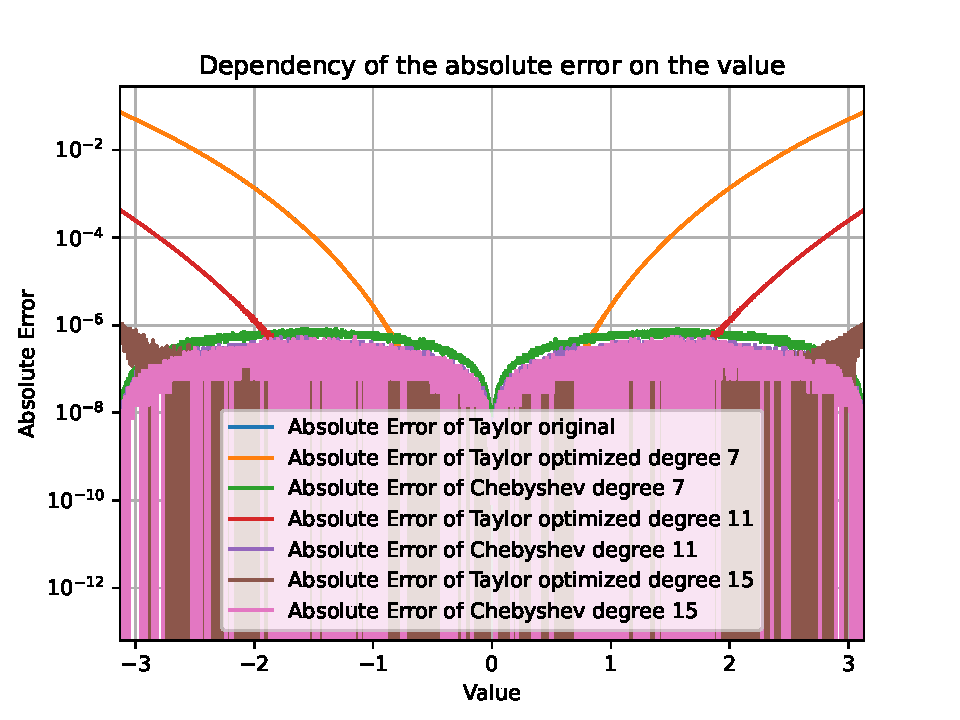
\includegraphics[width=\textwidth]{plots/accuracy/inc_abs_pi_001.pdf}
  \caption{Comparison of absolute error for various methods.}
  \label{fig:abs_error}
\end{figure}

\begin{figure}[h]
  \centering
  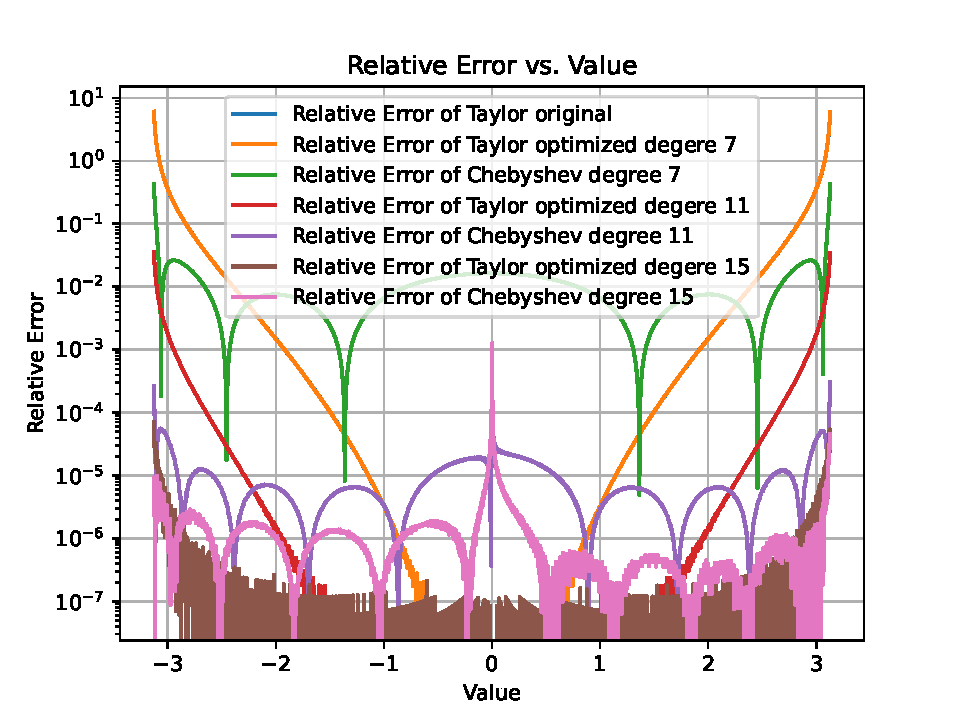
\includegraphics[width=\textwidth]{plots/accuracy/inc_rel_pi_001.pdf}
  \caption{Comparison of relative error for various methods. We compute relative error by comparing to \texttt{sin x} provided by \texttt{std} library.}
  \label{fig:rel_error}
\end{figure}

\begin{figure}[h]
    \centering
    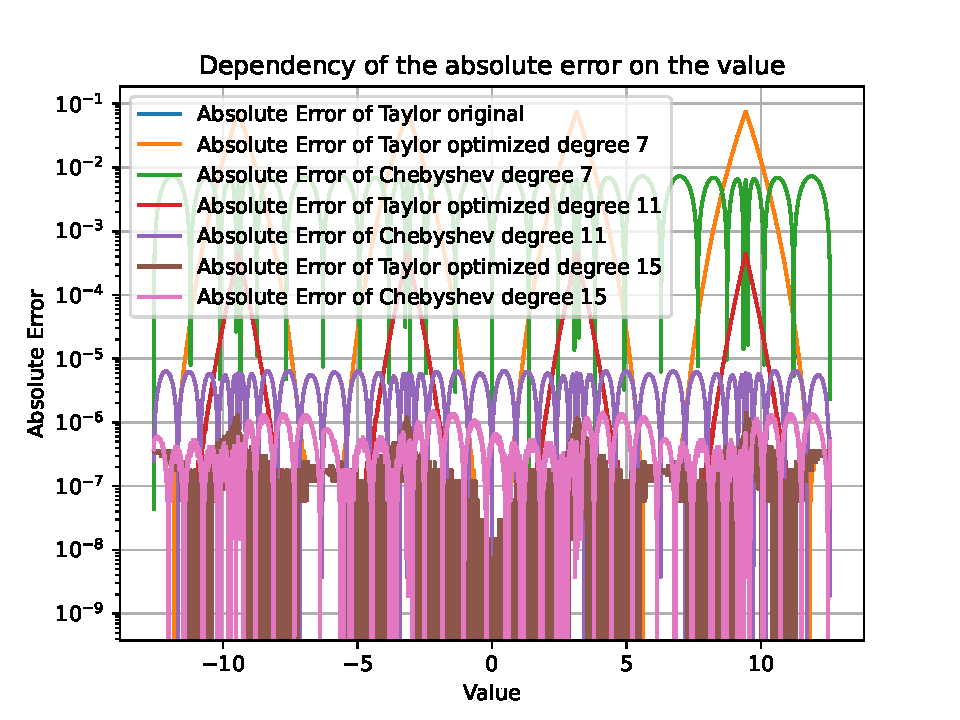
\includegraphics[width=\textwidth]{plots/accuracy/num_abs_two_pi_001.pdf}
    \caption{Comparison of absolute error for various methods.}
    \label{fig:abs_error_two_pi}
  \end{figure}

  \begin{figure}[h]
    \centering
    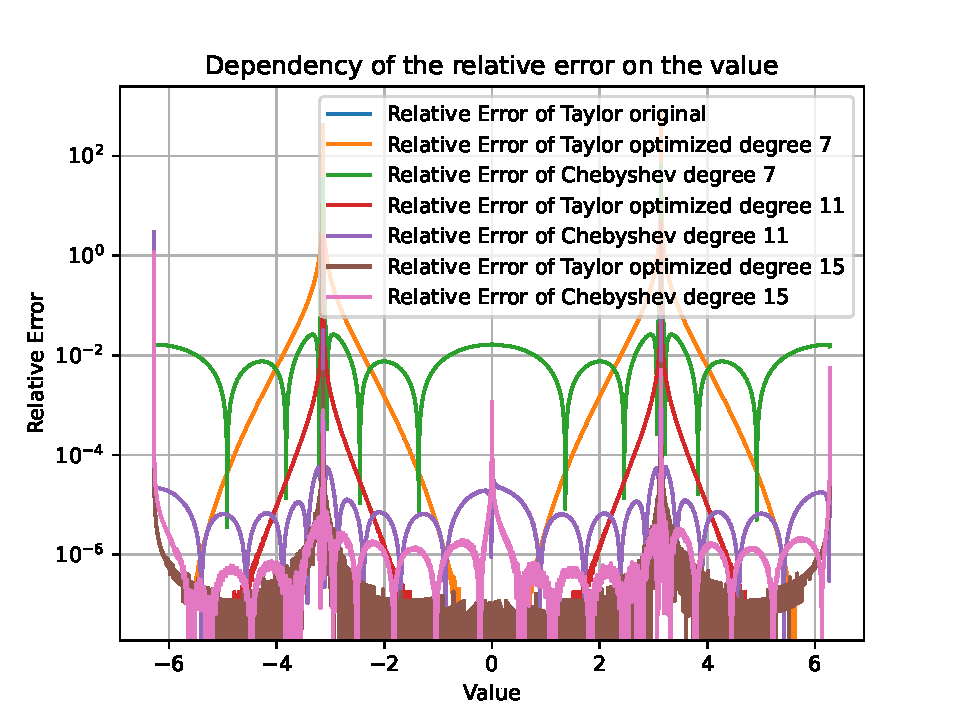
\includegraphics[width=\textwidth]{plots/accuracy/num_rel_two_pi_001.pdf}
    \caption{Comparison of relative error for various methods. We compute relative error by comparing to \texttt{sin x} provided by \texttt{std} library.}
    \label{fig:rel_error_two_pi}
  \end{figure}

\textbf{Performance.}
Based on Figure \ref{fig:perf_inc} and \ref{fig:cheb_vs_tay}, we can notice that Chebyshev approximation tends to be slower around one order of magnitude.
Similar, as we add more terms, the performance decreases, especially for the Chebyshev approximation.
We expected this since the time complexity is higher for the Chebyshev approximation.
In Figure \ref{fig:perf_orig_opt}, we also notice that the optimized Taylor series  is a little bit faster than the original one. Furthermore, the performance does not decrease that significantly.
Thus, we should use Taylor series with 11 terms in order to balance accuracy and performance.
For Chebyshev approximation, 11 terms provide sufficient accuracy (less than 1e-5).
\begin{figure}[h]
    \centering
    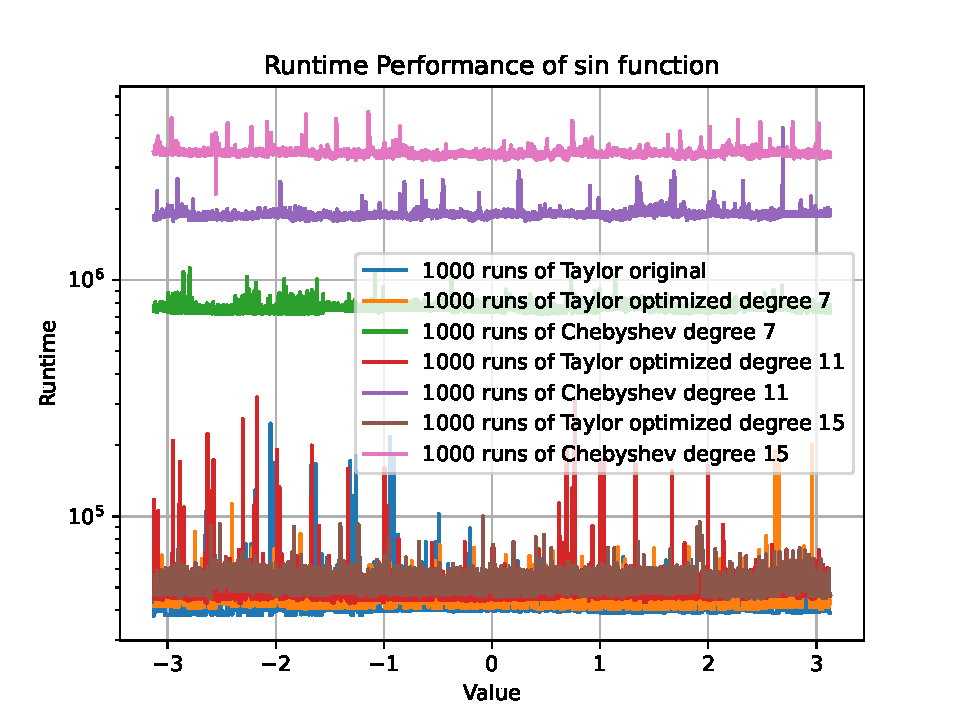
\includegraphics[width=\textwidth]{plots/performance/inc_rel_pi_001.pdf}
    \caption{Performance Comparison of Taylor series vs Chebyshev Approximation for 7, 11 and 15 terms.}
    \label{fig:perf_inc}
  \end{figure}

\begin{figure}[h]
    \centering
    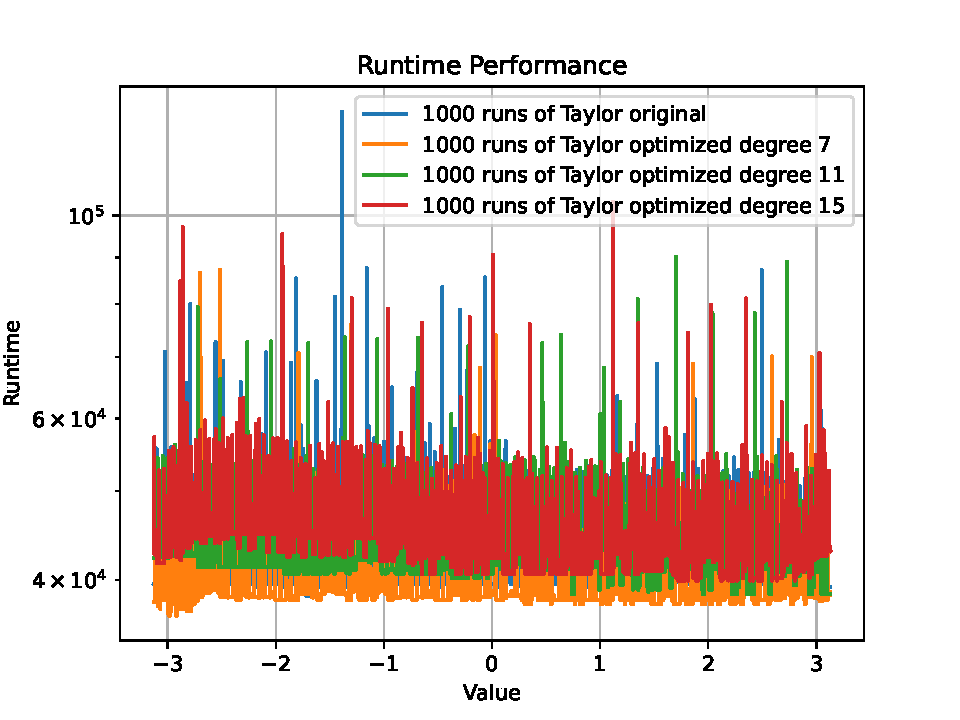
\includegraphics[width=\textwidth]{plots/performance/inc_rel_pi_tay_orig_vs_opt.pdf}
    \caption{Performance Comparison of Taylor series for 7, 11 and 15 terms.}
    \label{fig:perf_orig_opt}
\end{figure}

\begin{figure}[h]
    \centering
    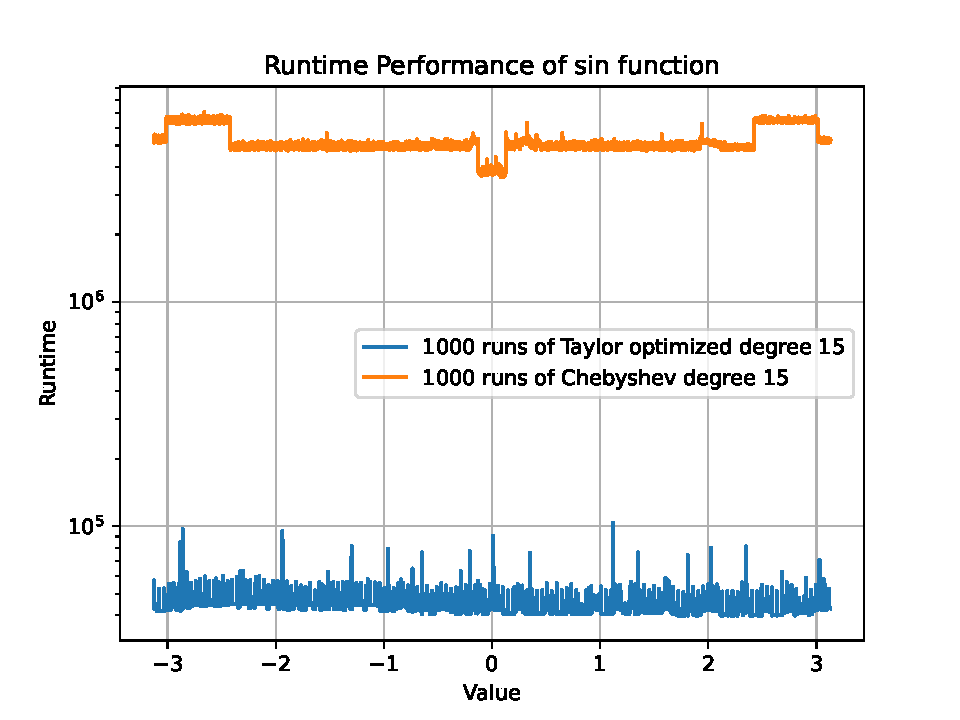
\includegraphics[width=\textwidth]{plots/performance/inc_rel_pi_tay_vs_cheb.pdf}
    \caption{Performance Comparison of Taylor series vs Chebyshev Approximation for 15 terms.}
    \label{fig:cheb_vs_tay}
\end{figure}

\bibliographystyle{plain}
\bibliography{refs}

\end{document}
